%%%%%%%%%%%%%%%%%%%%%%%%%%%%%%%%%%%%%%%%%%%%%%%%%%%%%%%%%%%%%%%%%%%%%%%%%%%%%%%%
% Es könnten Fragen kommen, warum nur 70%
% hier dann Bilder von der Uni und allen anderen Gebäuden, die wir nicht haben mappen können.
%%%%%%%%%%%%%%%%%%%%%%%%%%%%%%%%%%%%%%%%%%%%%%%%%%%%%%%%%%%%%%%%%%%%%%%%%%%%%%%%

\begin{frame}
 \frametitle{70\%}
    \begin{itemize}
	\item 10 * University
	\item Verschiebungen in OSM zu real (3, 7)
	\item umkreis ist nie perfekt
    \end{itemize}
\end{frame}

\begin{frame}
 \frametitle{}
  \Wider{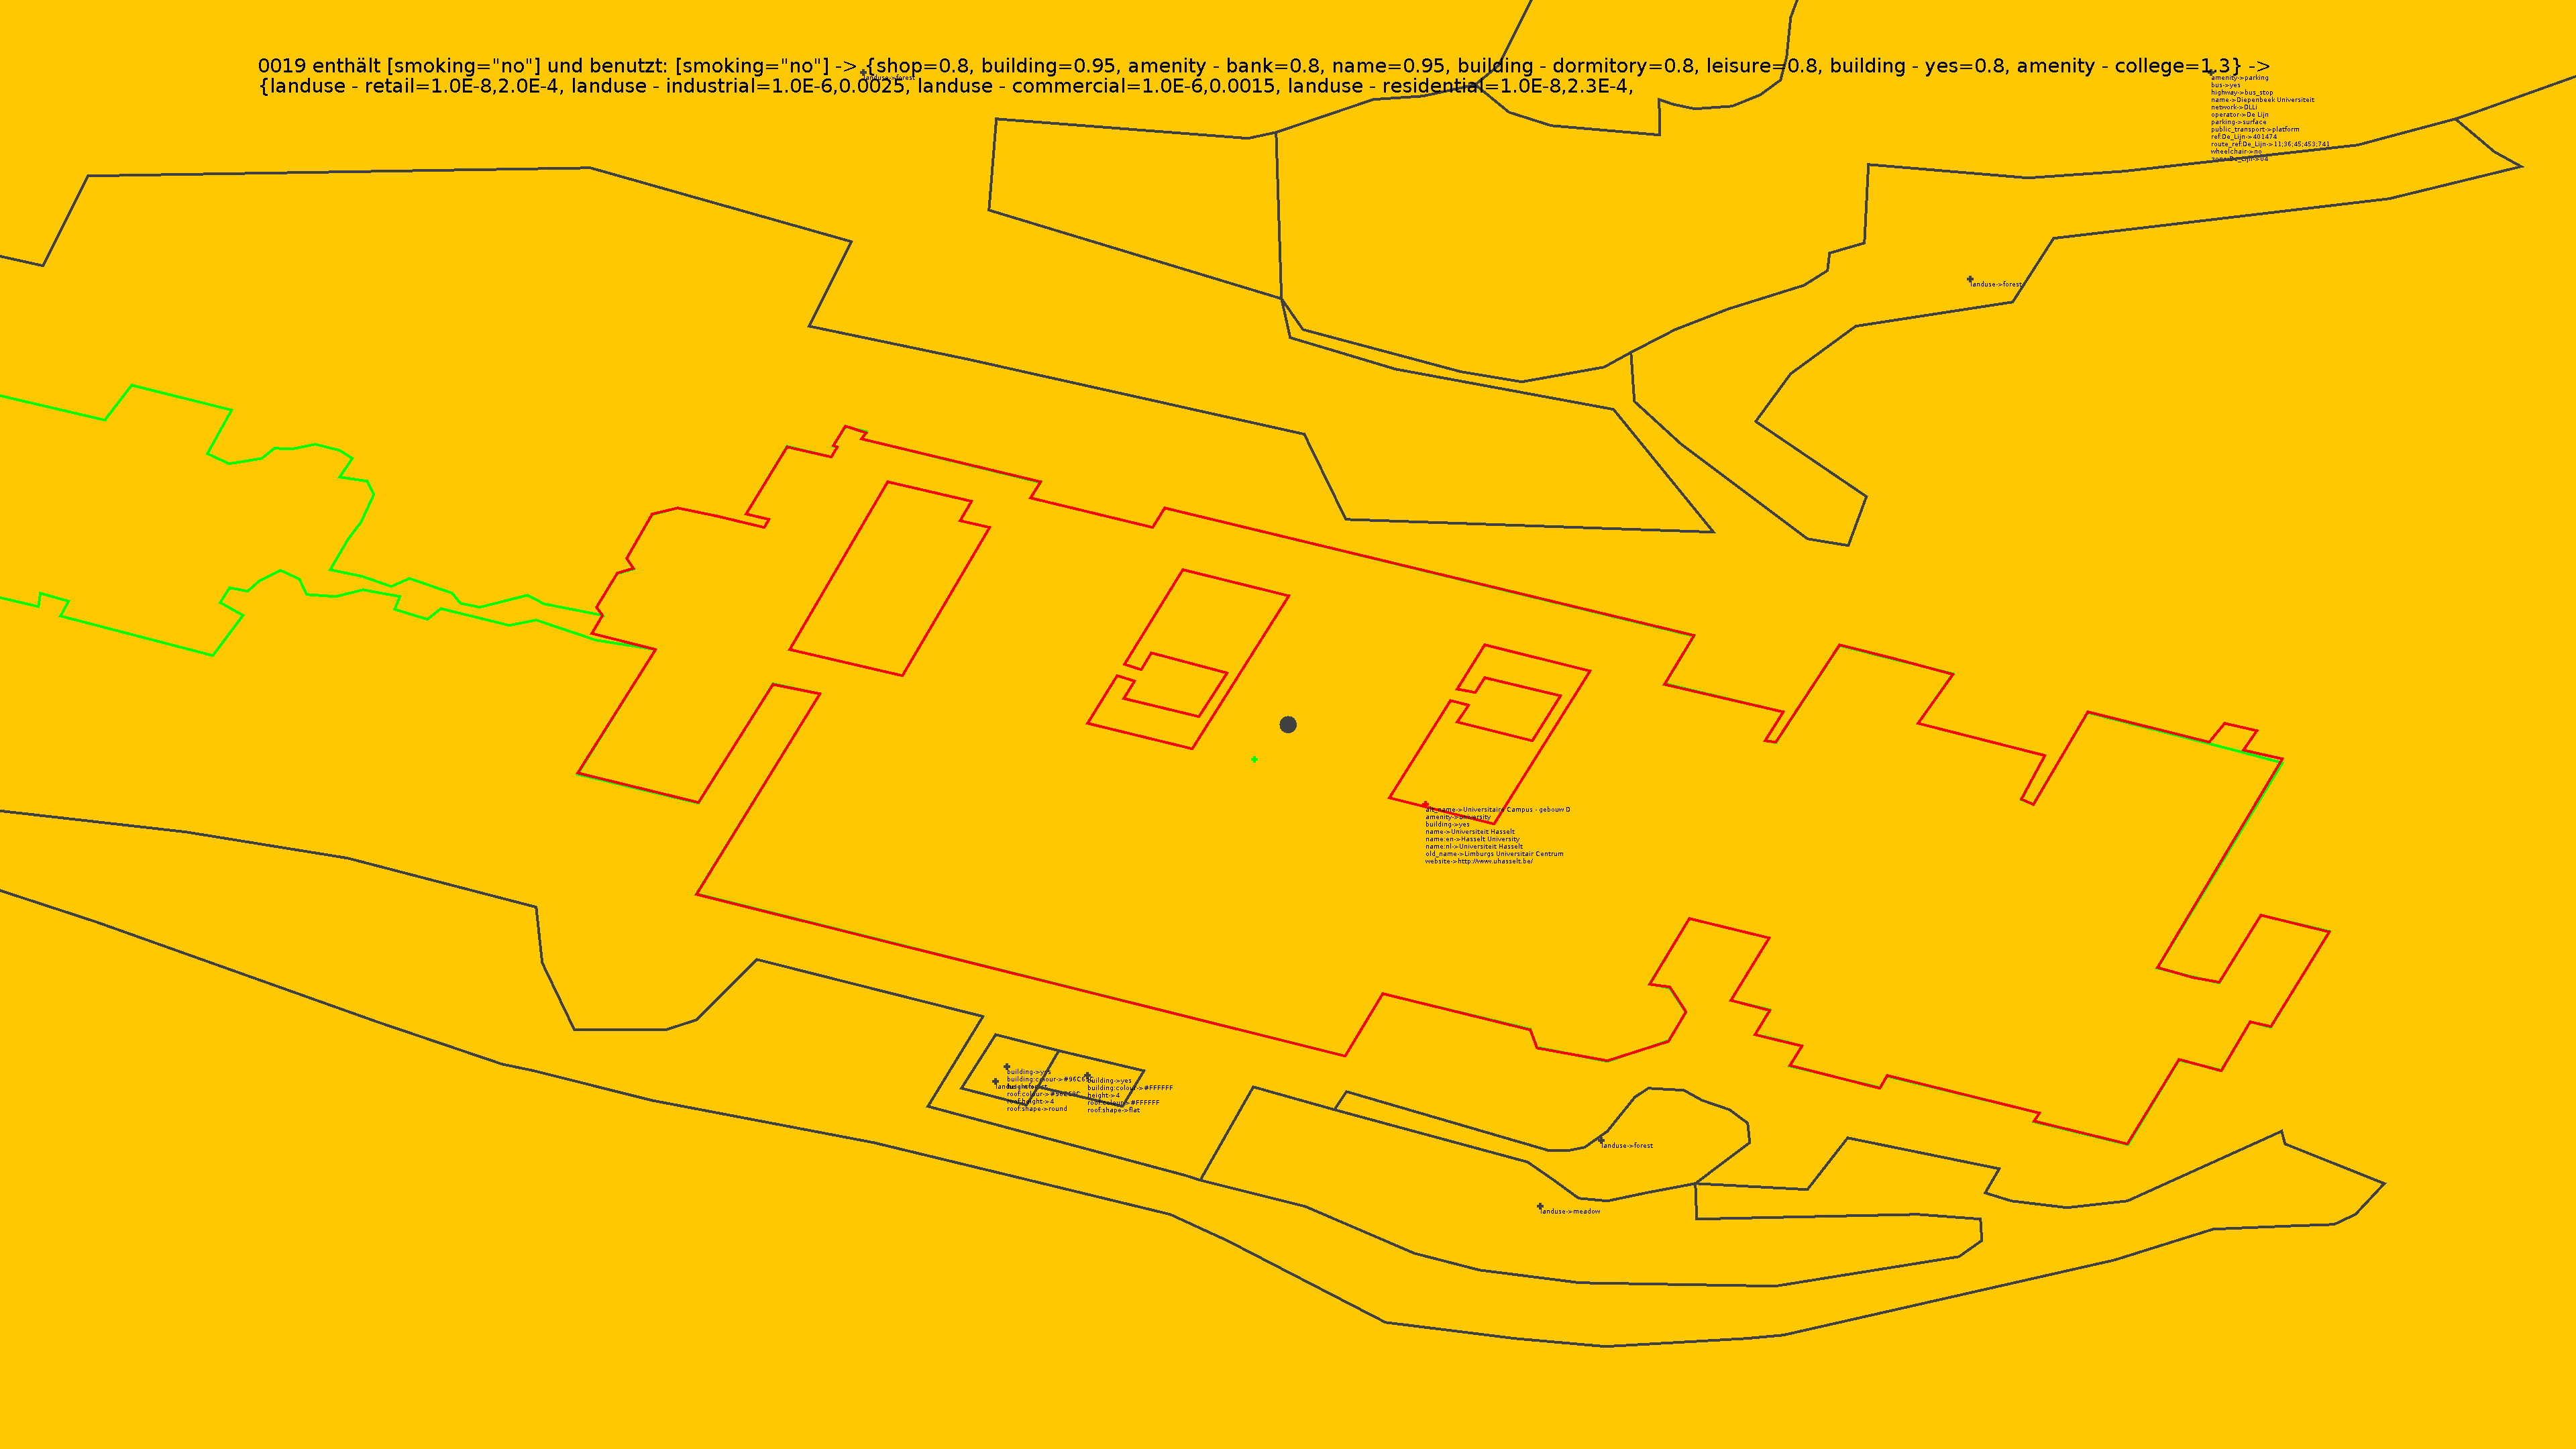
\includegraphics[width=\textwidth]{0019_big.png}}
\end{frame}


\begin{frame} %Distanzen mit Gewichtung
 \frametitle{Grundidee}
  \Wider{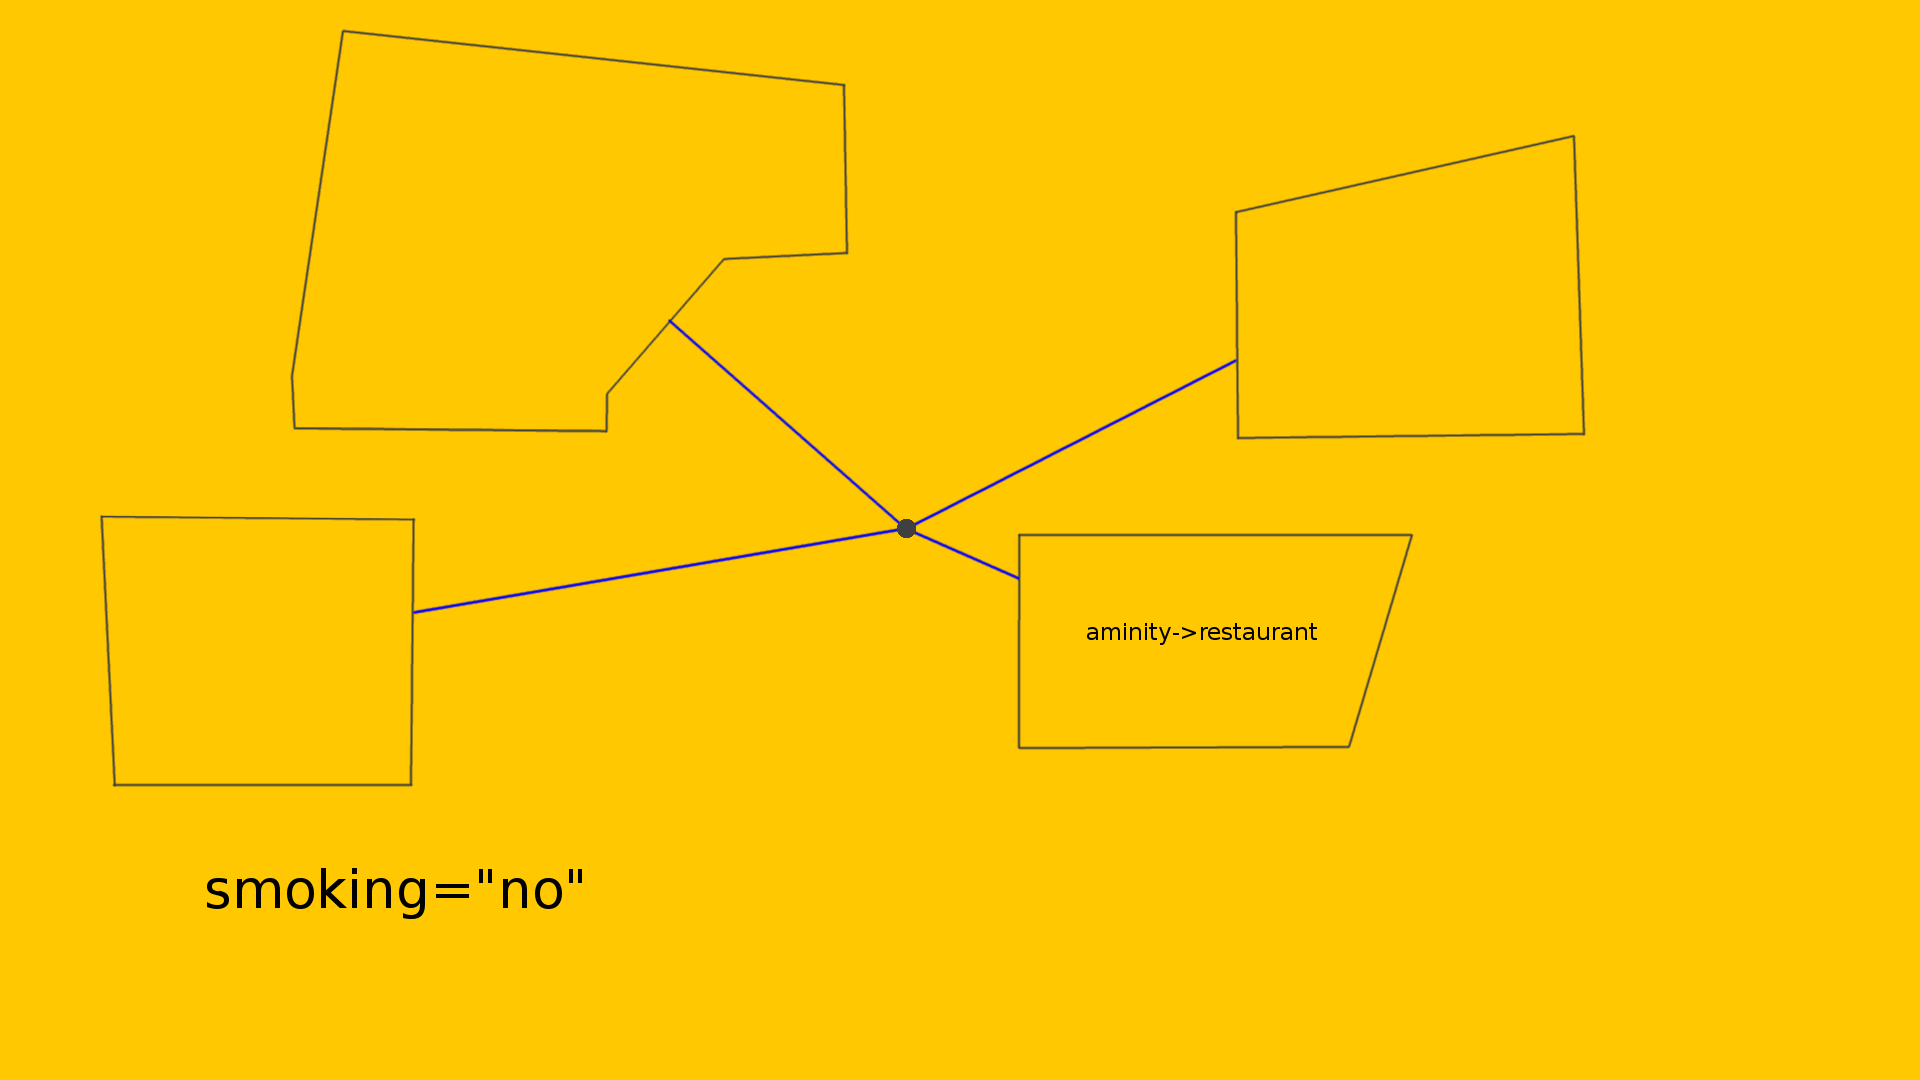
\includegraphics[width=\textwidth]{Funktionsweise_nachher}}
\end{frame}
